\documentclass[english, apj]{emulateapj}
\usepackage[T1]{fontenc}
\usepackage[latin9]{inputenc}
\usepackage{array}
\usepackage{rotating}
\usepackage{units}
\usepackage{textcomp}
\usepackage{amsmath}
\usepackage{amsbsy}
\usepackage{amstext}
\usepackage{graphicx}
\usepackage{url}
\usepackage{babel}
\usepackage{float}
%\usepackage{siunitx}
%\sisetup{output-exponent-marker=\ensuremath{\mathrm{e}}}
\usepackage[backref,breaklinks,colorlinks,citecolor=blue]{hyperref}
\usepackage[all]{hypcap}

\makeatletter

\newcommand{\msun}{\mbox{$\,{\rm M}_\odot$}}

\sloppy

\providecommand{\tabularnewline}{\\}

\begin{document}

\title{Cannibalism among the supermassive black holes}


\author{Charles Zivancev\altaffilmark{1}, Jeremiah P. Ostriker\altaffilmark{1,3}, Andreas H.W. K\"upper\altaffilmark{1,2}}
\altaffiltext{1}{Department of Astronomy, Columbia University, 550 West 120th Street, New York, NY 10027, USA}
\altaffiltext{2}{Hubble Fellow}
\altaffiltext{3}{Princeton University, New Jersey, USA}
\email{Correspondence to: csz2104@columbia.edu}




\begin{abstract}

\end{abstract}


\keywords{Galaxy: kinematics and dynamics}




\section{Introduction}\label{sec:introduction}
What happens to the massive black holes centrally located in galaxies when those galaxies merge with others?  There are three possibilities: they merge, they are ejected, or they remain in orbit in the merged galaxy.  Combinations of these options are also possible with the spin induced kick at merger leading to an ejection or extended orbit of the merged black hole.  We now know from pulsar timing measurements (ADD REFERENCES) that the gravitational wave background is probably too low for most galaxy mergers (mass-weighted) (but see \cite{2018NatCo...9..573M}) to lead to BH mergers, but the outcome remains uncertain.  We will argue in this paper that a very common outcome--especially for the lower mass black holes--is for the injected objects to remain as orbiting X-ray sources in normal massive galaxies waiting to be identified by current observational techniques.

A majority of all galaxies with masses $>10^8\msun$ at $z=0$ are believed to host super-massive black holes (SMBHs) in their cores.  What is the ultimate fate of the supermassive black holes (SMBH) resident at the centers of these massive galaxies?  For the galaxies themselves we know that mergers are frequent from the observed (VAN DOKKUM PAPERS??) evolution of the size and mass of these systems.  But assuming that all galaxy mergers lead to SMBH mergers overpredicts the observations of gravitational waves from the pulsar timing arrays (PTAs) (\citet{2015ApJ...799..178K}, \citet{2014ApJ...789..156M}, \citet{2008MNRAS.390..192S}, \citet{2013MNRAS.433L...1S}, \citet{2018ApJ...856...42S}, \citet{2009MNRAS.394.2255S}, \citet{2018arXiv180403143I}).  But we do not often see multiple SMBHs at the centers of massive ellipticals.  So, what does happen?  One paper (\citet{2018MNRAS.473.3410R}) has indicated that dynamical interactions among multiple black holes, which eject a non-negligible fraction of the mass, may solve this problem.  The present paper also addresses this purported dynamical solution, focusing attention on the large fraction of lower mass black holes that remain to be detected as they orbit in massive galaxies.  What we argue in this paper is that as a result of the N-body interactions among the infalling black holes some are ejected, some remain in extended orbits and some (the few most massive ones) do in fact merge but we do not exceed the PTA limits, and the orbiting ones should be detectable via their ability to accrete gas and emit radiation.

Here we look at the merger history of 13 exemplary galaxies across the galaxy mass spectrum extracted from a cosmological simulation of hierarchical structure formation. We investigate how, after merging with incoming galaxies, SMBHs diffuse into the cores of the hosts and interact with the resident black hole. We show that gravitational interactions of multiple SMBHs are most probable in high-mass galaxies with $10^{12} \msun < M < 10^{13} \msun$. Galaxies with lower masses have too few mergers with SMBH hosting galaxies. Galaxies with higher masses are more extended, making dynamical friction processes less efficient and hence failing to drive SMBHs into the host galaxy core.

This paper is organized as follows: in Section \ref{sec:methods} we describe the cosmological simulation from which we use the merger history to set up our idealized numerical simulations. We present the few-body integration code, \textsc{AR-Chain} that we used for our simulations of SMBH dynamics, and the modifications we made to this code in order to deal with a host galaxy's gravitational potential. In Section \ref{sec:results}, we show the results of our XX exemplary simulations of galaxies growing with time and acquiring new SMBHs. We analyze how the SMBHs are driven into the core of their new host galaxies and how interaction with the host black hole leads to near-ejections or mergers. The final Section \ref{sec:conclusions} contains a discussion of the result and our conclusions.


\section{Methods}\label{sec:methods}
%\begin{figure*}[htbp]
%\begin{center}
%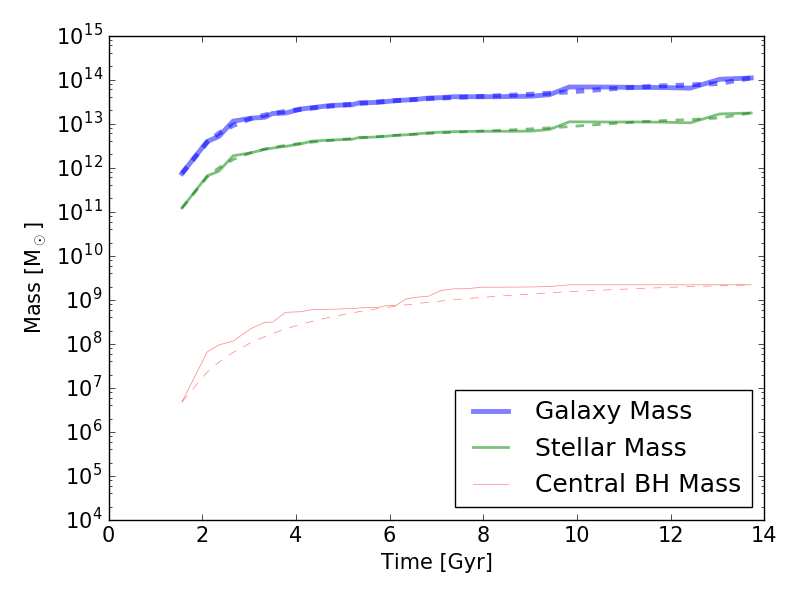
\includegraphics[width=0.45\textwidth]{plots/Masses_plot_galaxy_1.png}
%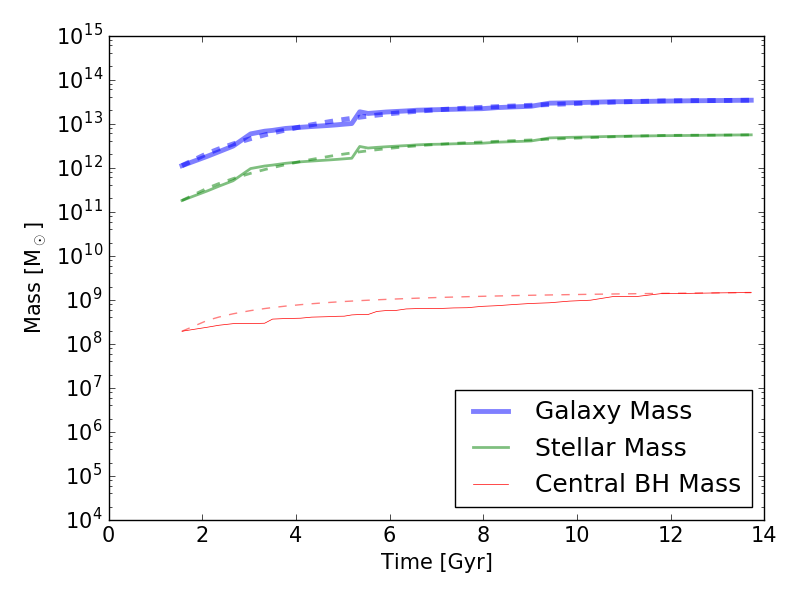
\includegraphics[width=0.45\textwidth]{plots/Masses_plot_galaxy_65.png}\\
%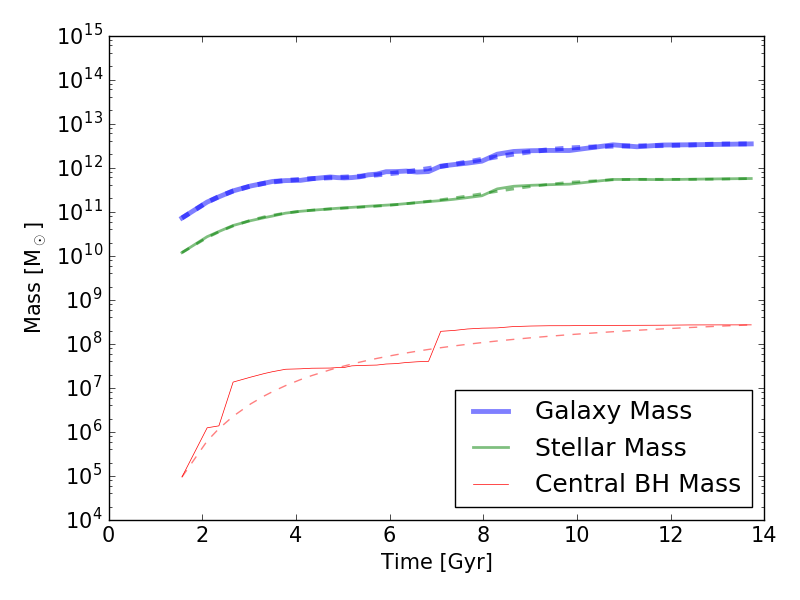
\includegraphics[width=0.45\textwidth]{plots/Masses_plot_galaxy_187.png}
%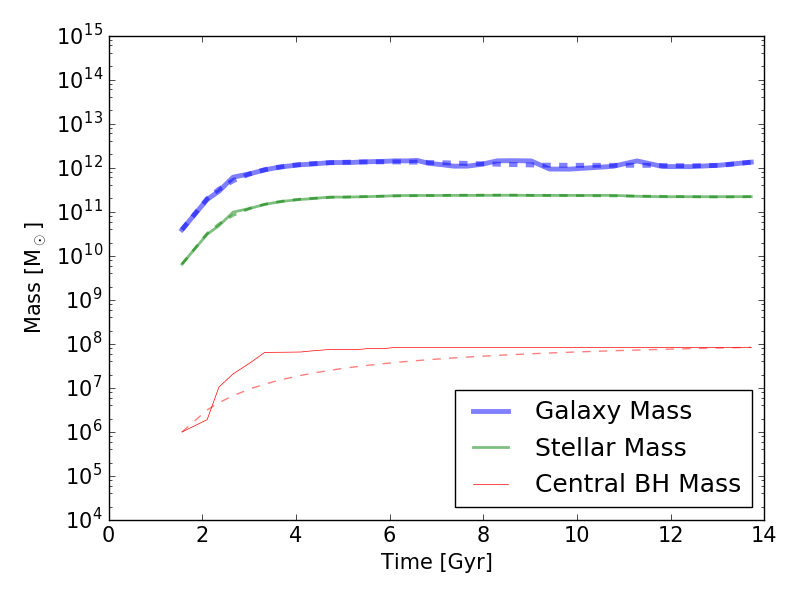
\includegraphics[width=0.45\textwidth]{plots/Masses_plot_galaxy_217.png}\\
%\caption{default}
%\label{default1}
%\end{center}
%\end{figure*}

\subsection{Overview of simulation}
Our simulations focus on elliptical galaxies with central SMBHs. The galaxies were given a background potential based on the Ostriker-Stone profile (\citet{2015ApJ...806L..28S}), which is a three-parameter potential-density pair, whose quantities such as density, potential, and binding energy can be written in closed form.  The galaxies were evolved from $4 > z > 0$.  Orbiting black holes were periodically introduced into the "host" galaxy and their dynamical interaction with the background potential and central SMBH were followed, as described further below.

For the numerical simulations presented here, we used a modified version of the algorithmic chain integrator \textsc{AR-Chain} developed by \citet{2006MNRAS.372..219M}. It uses algorithmic chain regularization for high-precision integration of few-body dynamics, and is capable of handling velocity-dependent forces efficiently. It includes relativistic post-Newtonian terms up to order PN2.5 \citep{2008AJ....135.2398M}.


\subsection{Merger tree}
Our merger tree data came from two sources:
\begin{itemize}
\item Galactic merger tree data from simulations of \citet{2012MNRAS.425..641L} (hereafter Lackner12), which was centered on galaxies at each redshift slice, providing information on the galaxies' stellar mass, dark matter mass, central BH, and any orbiting black holes within the galaxy.
\item SMBH evolution simulations of \citet{2015ApJ...799..178K} (hereafter Kulier15), which used the large-scale hydrodynamical galaxy simulations outlined in \citet{2011ApJ...741...99C, 2011ApJ...742L..33C, 2012ApJ...753...17C, 2012ApJ...748..121C, 2013ApJ...770..139C}.  The data was centered around SMBHs at each redshift slice from $4 > z > 0$, giving information for each SMBH's seed mass, accreted and seed mass, its host galaxy (categorically defined), the stellar mass in its host galaxy, and time after z=4 at which the BH entered the host galaxy (if it is not the central BH).
\end{itemize}

The merger tree data from Lackner12 and Kulier15 provided 1,830 galaxies in total.  However, not all the galaxies were suitable for our simulations.  We placed further requirements as follows:
\begin{itemize}
\item The galaxies had to exist through the entire simulation ($4 > z > 0$).  If they merged with other galaxies, they had to have been the "surviving" galaxy at each merger.
\item They had to have accumulated orbiting black holes by z = 0.
\end{itemize}

The Kulier15 merger tree collected black holes entering galaxies during the simulation and noted the time after z=4 at which they entered their host galaxy.  Nothing further was done with them, so each galaxy had a "running list" of other galaxies/BHs orbiting them at z=0.  Clean up this paragraph.

After finding our subject galaxies, we curve-fit their total masses as a function of time using a $7^{th}$-order polynomial fit, so as to be able to use their masses in the AR-Chain code.  Additionally, we curve-fit each galaxy's accreted+seed central black hole mass to exponential functions of time.

The following cosmological parameters were used in the simulations of both Lackner12 and Kulier15:   $\Omega_M = 0.28$, $\Omega_b = 0.046$, $\Omega_\Lambda = 0.72$, $\sigma_8 = 0.82$, $H_0 = 100h^{-1}Mpc^{-1} = 70 km s^{-1} Mpc^{-1}$, and $n = 0.96$.

\subsubsection{Galactic Stellar Mass Adjustment}
Lackner12 noted that the efficiency of star formation in their simulations, defined as $f_*=M_*/M_{DM}(\Omega_{DM}/\Omega_b)$, was approximately 0.6.  Compared with the expected range of $0.10 \lessapprox f_* \lessapprox 0.15$ that they referenced from \citet{2012ApJ...746...95L}, their stellar masses were a factor of roughly 4 times greater.  We used observational data from \citet{2018AstL...44....8K}, in particular Figure 11, to rescale the stellar masses to the observed range.
\begin{figure}[h!]
\begin{center}
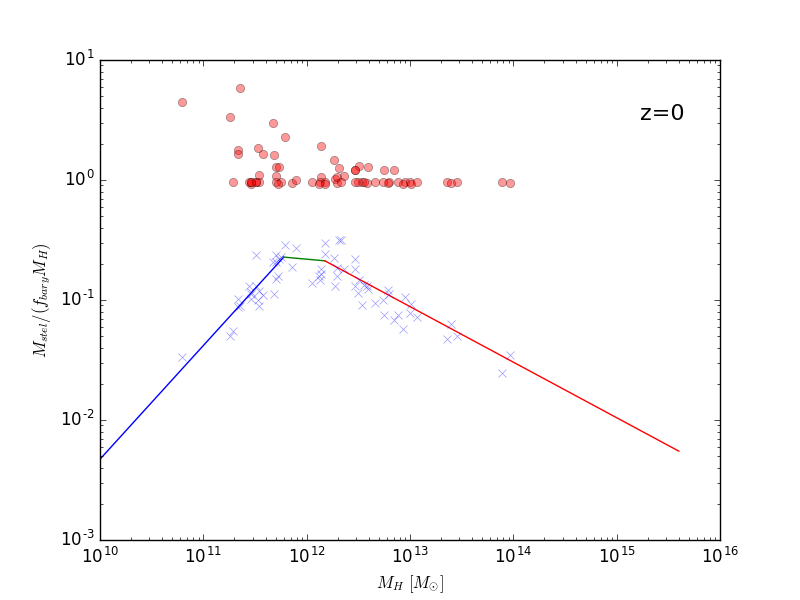
\includegraphics[width=0.45\textwidth]{plots/stellar_to_halo_ratio.png}
\caption{Original and rescaled stellar masses}
\label{fig:stellar1}
\end{center}
\end{figure}

\subsection{AR-Chain code}
Summary of the code and the modifications we made.

\subsubsection{Galaxy background potential}
For our simulations, the Stone-Ostriker profile (\citet{2015ApJ...806L..28S}), which is a three-parameter potential-density pair, whose quantities such as density, potential, and binding energy can be written in closed form.  It is essentially an analytic form of a finite, cored isothermal mass distribution:
\begin{equation} \label{jerry}
\rho(r) = \frac{\rho_c}{(1+r^2/r_{c}^2)(1+r^2/r_{h}^2)}
\end{equation}
Here $\rho_c$ is the central density, $r_c$ is the core radius, and $r_h$ is the outer halo radius.

In order to parametrize this profile, $r_c$ was given an initial value of 100 pc, which is reasonable for a cored massive system.  To calculate $r_h$, we began by using the stellar mass to calculate the velocity dispersion at the galaxy's effective radius.  In Kulier12, the galaxy's effective radius $R_{e}$ and velocity dispersion $\sigma(R_e)$ at the effective radius are:
\begin{equation} \label{re}
R_{e} = 2.5 kpc\left(\frac{M_*}{10^{11}M_{\odot}}\right)^{0.73}(1+z)^{-0.98}
\end{equation}
\begin{equation} \label{sig}
\sigma(R_{e}) = 190km/s\left(\frac{M_{*}}{10^{11}M_{\odot}}\right)^{0.2}(1+z)^{0.47}
\end{equation}

We can then equate the value for $\sigma({R_e})$ obtained from Equation \ref{sig} to the analytic expressions for $\sigma(R_{e})$ in the Stone-Ostriker profile (Eqns 9 and A1-A4).  The only unknown is $r_h$, which we can solve for using a simple recursive Newton method.  Whether $\sigma_{near}$ or $\sigma_{far}$ is used from Stone-Ostriker is determined by whether $R_e$ is less than or greater than $\sqrt{r_c r_h}$.

The central density, $\rho_c$, can be found from Equation 5 in Stone-Ostriker:
\begin{equation} \label{rhoc}
M_{tot} = \frac{2\pi^2r_{c}^2r_{h}^2\rho_c}{r_h+r_c},
\end{equation}
where $M_{tot}$ is the total dark matter mass.

At each iteration in the code, $r_h$ is updated according to the stellar mass and Equations \ref{re} and \ref{sig}.  The core radius, $r_c$, is recalculated only if an orbiting black hole gets within $r_c$.  The work done by diffusion, as described in Section \ref{psd} is calculated, the total potential energy is updated, and $r_c$ is solved for from Equation 8 in Stone-Ostriker.

\subsubsection{Phase-space diffusion} \label{psd}
Weak encounters with background stars will let the SMBHs diffuse through phase space while they are orbiting within the gravitational potential of the galaxy. The diffusion can be expressed as change in velocity of an SMBH by $\Delta \vec{v}$ per unit time. We can split this change into a component along the direction of motion of the SMBH, and one perpendicular to that. Following \citet{2008gady.book.....B}, the diffusion coefficients can be expressed as 
\begin{eqnarray}\label{eq:df}
D[\Delta v_\parallel] & = & -\frac{4\pi G^2\rho(r)M_\bullet\ln\Lambda}{\sigma^2}f(\chi),\\
D[(\Delta v_\parallel)^2] & = & \frac{4\sqrt{2}\pi G^2\rho(r)M_\bullet\ln\Lambda}{\sigma}\frac{f(\chi)}{\chi},\\
D[(\Delta \vec{v}_\bot)^2] & = & \frac{4\sqrt{2}\pi G^2\rho(r)M_\bullet\ln\Lambda}{\sigma}\left[\frac{\mbox{erf}(\chi)-f(\chi)}{\chi}\right],
\end{eqnarray} 
where $\Delta v_\parallel \equiv \Delta \vec{v}\cdot\vec{v}/v$ is the velocity change in direction of motion, and $\Delta \vec{v}_\bot \equiv \Delta \vec{v} - \Delta v_\parallel \cdot\vec{v}/v$ is the velocity change perpendicular to the direction of motion. Here, $M_\bullet$ is the mass of the black hole, and $\chi = \frac{v}{\sqrt{2}\sigma(r)}$. The function $f(\chi)$ is given by 
\begin{equation}
f(\chi) \equiv \frac{1}{2\chi^2}\left(\mbox{erf}(\chi)-\frac{2\chi}{\sqrt{\pi}}\exp\left(-\chi^2\right)\right).
\end{equation}
We approximate the factor $\Lambda$ in the Coulomb logarithm as
\begin{equation}
\Lambda \equiv \left(\frac{M_{NSC}}{M_\bullet}\right)\left(\frac{r}{r_h}\right).
\end{equation}
We can identify Equation \ref{eq:df} as the dynamical friction term. The second term introduces a variance of the friction term, and even allows the SBHs to be accelerated when the velocity of a SBH gets sufficiently small. The third term introduces a change in velocity perpendicular to the direction of motion of the SBH. It is a randomly oriented vector, and hence causes the SBHs to execute a random walk in phase space. The last two terms will establish that the SBHs are ultimately in energy equipartition with the background stars.
The velocity changes $\Delta v_\parallel$ and $\Delta\vec{v}_\bot$ per unit time $\Delta t$ can be computed with the above equations. Both changes are normally distributed, where the mean, $\mu$, and the variance, $\Sigma$, of the distributions are given by
\begin{eqnarray}
\mu_\parallel &=& D[\Delta v_\parallel]\Delta t,\\
\Sigma_\parallel &=& D[(\Delta v_\parallel)^2]\Delta t,\\
\mu_\bot &=& 0,\\
\Sigma_\bot &=& D[(\Delta \vec{v}_\bot)^2]\Delta t.
\end{eqnarray}
We compute the diffusion coefficients for each black hole at each time step, and modify its velocity on a Monte Carlo basis. For each time step we draw a random orientation before adding the perpendicular velocity change to the respective SBH. Hence, the SBH's modified velocity, $v_f$, is computed using
\begin{eqnarray}
\vec{v}_f &=& \vec{v}_0 + \Delta v_\parallel \hat{v}_\parallel + \Delta v_\bot \hat{v}_\bot,\\
\Delta v_\parallel &=& \mathcal{N}(\mu_\parallel, \Sigma_\parallel),\\
\Delta v_\bot &=& \mathcal{N}(\mu_\bot, \Sigma_\bot).
\end{eqnarray}
The change of energy, $\mbox{d}E_{BH}$, of the orbiting black hole due to phase-space diffusion is given back to the stellar background potential, with $\mbox{d}E = -\mbox{d}E_{BH}$. As a consequence of this energy transfer, inspiralling black holes will cause an expansion of the NSC. For this purpose we calculate the change in potential energy, $\mbox{d}W$, of the stellar system using
\begin{eqnarray}
E &=& T + W = \frac{1}{2}W,\\
\mbox{d}W &=& -2\,\mbox{d}E_{BH},
\end{eqnarray}
where we made use of the virial theorem $2T+W =0$. With this change in potential energy we can calculate a new radius for the stellar background potential at each integration step. For the Plummer sphere the new scale radius can be calculated as
\begin{equation}
a_{new} = a\left(1+\frac{32a\,\mbox{d}W}{3\pi GM_{NSC}^2}\right)^{-1}.
\end{equation}

\subsubsection{Gravitational wave recoils}
The code \textsc{AR-Chain} includes post-Newtonian terms up to order 2.5. The SMBHs can therefore merge via gravitational wave emission. We include gravitational wave recoils following the prescription outlined in Kulier15, which is based on the fitting formula by \citet{2012PhRvD..85h4015L}. To save computational time, we assume that a merger will be inevitable when the separation between two SBHs becomes smaller than 1.0 Schwarzschild radius. At the moment of the merger, we assume that the spin vectors of the two SBHs are randomly aligned. This results in kick velocities of up to several thousand km\,s$^{-1}$, with a median kick of $\approx 290$\,km\,s$^{-1}$. Since our simulations focus on NSC with relatively low escape velocities, this implies that a majority of the merging SBHs escape from the NSCs. 

Black holes can also eject each other via strong three-body interactions. We remove SBHs from the simulations once they move beyond 1\,kpc from the NSC, assuming that it will take them more than a Hubble time to find their way back into the center of the host galaxy.

\subsection{Simulation setup}
Note to discuss:  Injection, merging, escape, effective radius, set of galaxies

Using the merger tree data, orbiting black holes were injected into its host galaxy at redshift z, at a distance from the galactic center of $R_{e}$ (Eqn. \ref{re}).  Their initial velocity was arbitrarily chosen to be circular, $v_c = \sqrt{M(R_e)/R_e}$, with $v_x$, $v_y$, and $v_z$ randomly chosen.  Note: we only inject the BHs into the simulation that have a $t_{fric}$ smaller than 100 times the Hubble time.


\subsection{Description of Simulations}
\begin{table*}
\centering
\caption{Galaxy characteristics}
\begin{tabular}{c| c c| c c| c c}
 & \multicolumn{2}{c}{$M_{gal}$ [$M_{\odot}$]} & 
\multicolumn{2}{c}{$M_{*}$ [$M_{\odot}$]} & 
\multicolumn{2}{c}{$M_{BH}$ [$M_{\odot}$]} \\
\hline
Galaxy & Init & Final & Init & Final & Init & Final \\
 \hline
A & $7.42\times10^{11}$ & $1.09\times10^{14}$  & $1.22\times10^{11}$ & $1.75\times10^{13}$ & $4.80\times10^{6}$ & $2.19\times10^{9}$\\
B & $1.11\times10^{12}$ & $3.41\times10^{13}$ & $1.80\mathrm{3}{11}$ & $5.58\times10^{12}$ & $1.94\times10^{8}$ & $1.46\times10^{9}$\\
C & $7.23\times10^{10}$ & $3.48\times10^{12}$ & $1.18\times10^{10}$ & $5.68\times10^{11}$ & $9.47\times10^{4}$ & $2.70\times10^{8}$\\
D & $3.92\times10^{10}$ & $1.34\times10^{12}$ & $6.47\times10^{9}$ & $2.20\times10^{11}$ & $9.95\times10^{5}$ & $8.32\times10^{7}$\\
\end{tabular}
\end{table*}





\section{Results}\label{sec:results}
\begin{figure}[H]
\begin{center}
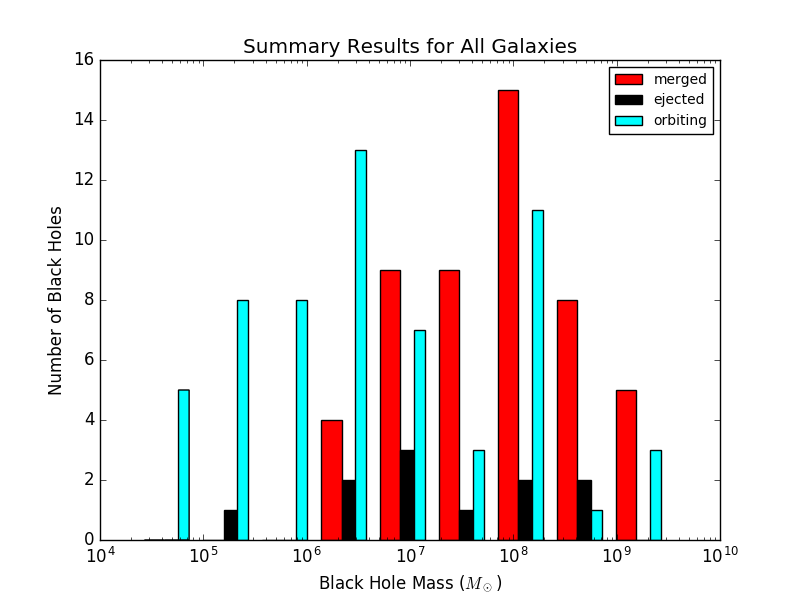
\includegraphics[width=0.45\textwidth]{plots/Summary_Results_All_Galaxies.png}
\caption{Histogram of merged, ejected, and orbiting SMBHs}
\label{fig:meosmbh}
\end{center}
\end{figure}

\begin{table*}
\centering
\caption{SMBH statistics}
\begin{tabular}{c| c |c |c}
Galaxy & Infalling SMBHs & SMBHs with $t_{fric}<100\,t_H$ & Mergers \\
\hline
A & 206 & 19 & 4 \\
B & 29 & 12 & 4 \\
C & 3 & 3 & 2 \\
D & 4 & 4 & 2 \\
\end{tabular}
\end{table*}

\begin{figure*}[htbp]
\begin{center}
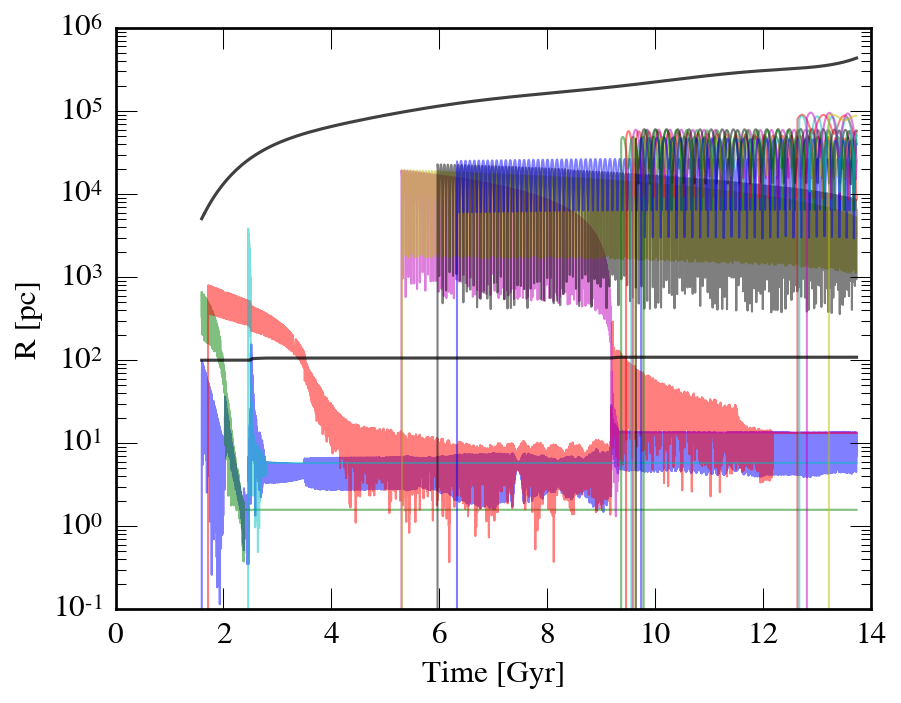
\includegraphics[width=0.45\textwidth]{plots/radius_A.png}
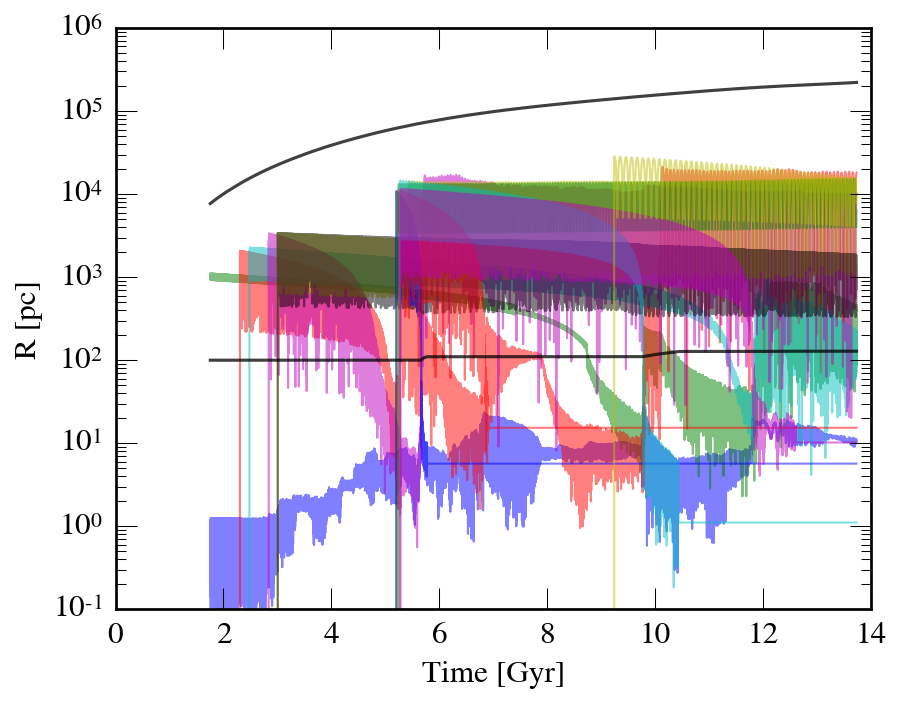
\includegraphics[width=0.45\textwidth]{plots/radius_B.png}\\
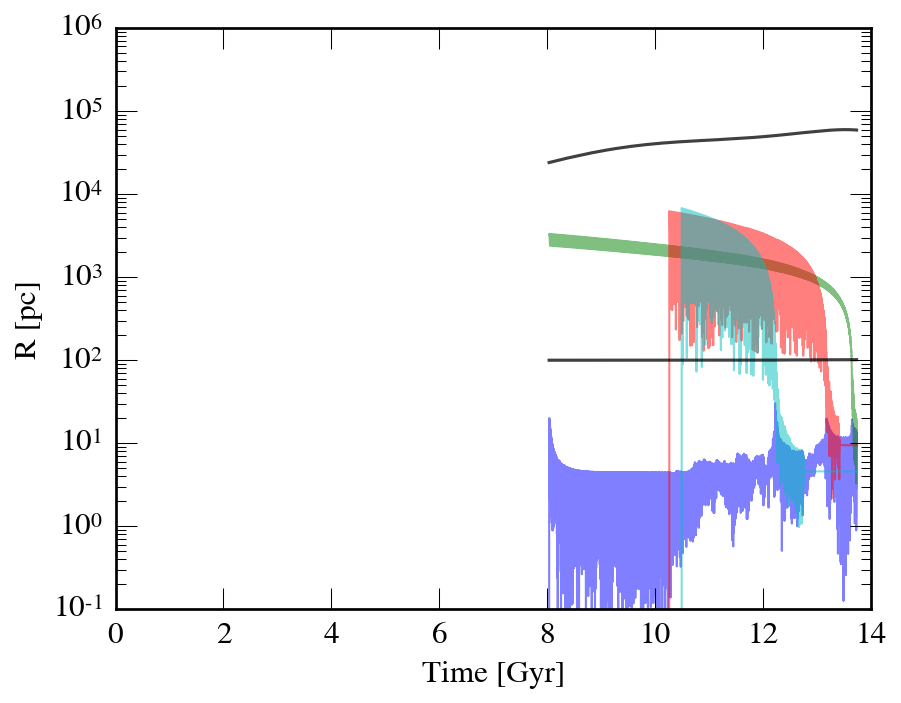
\includegraphics[width=0.45\textwidth]{plots/radius_C.png}
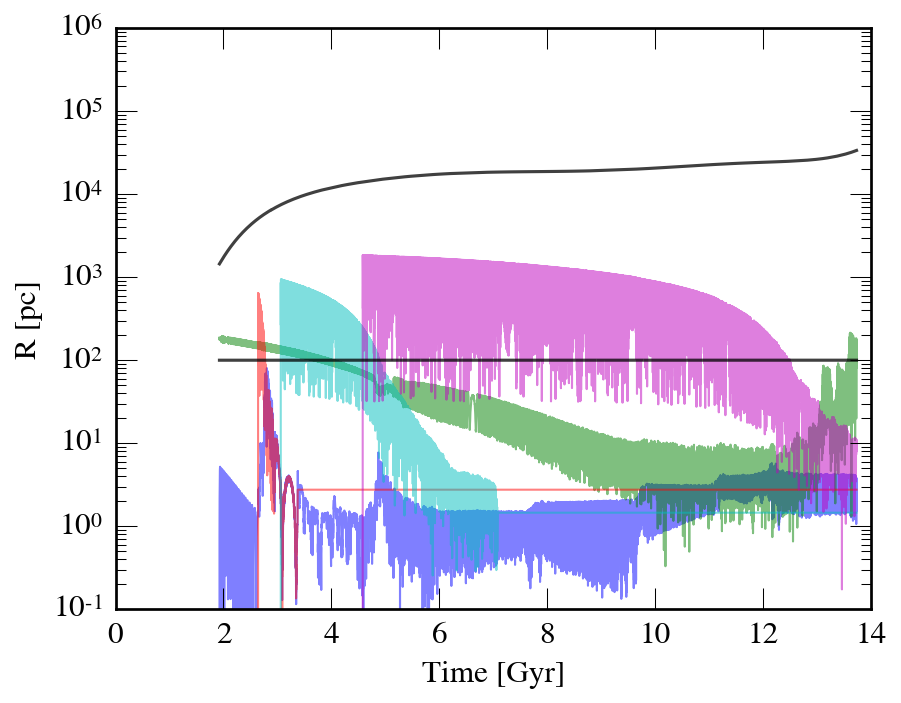
\includegraphics[width=0.45\textwidth]{plots/radius_D.png}\\
\caption{default}
\label{default2}
\end{center}
\end{figure*}

\begin{figure*}[htbp]
\begin{center}
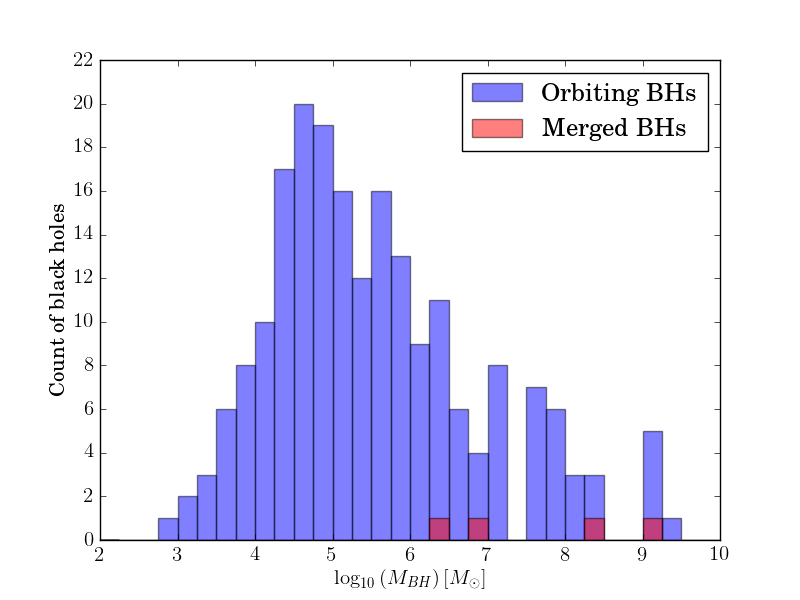
\includegraphics[width=0.45\textwidth]{plots/orbiting_bh_mass_histogram_gal_1.png}
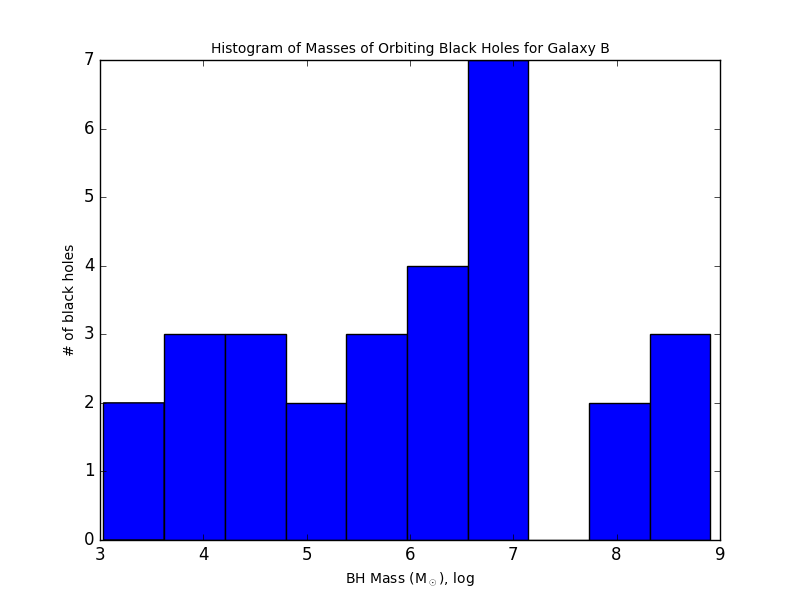
\includegraphics[width=0.45\textwidth]{plots/orbiting_bh_mass_histogram_gal_65.png}\\
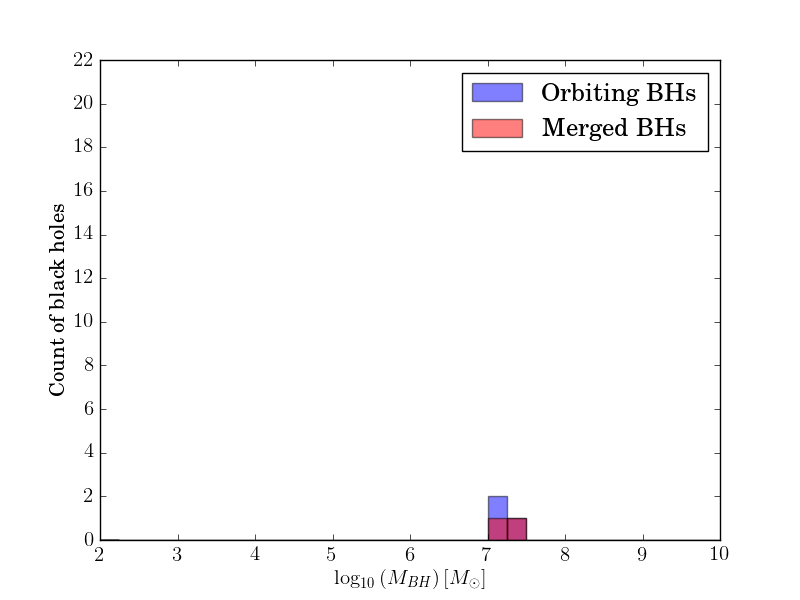
\includegraphics[width=0.45\textwidth]{plots/orbiting_bh_mass_histogram_gal_187.png}
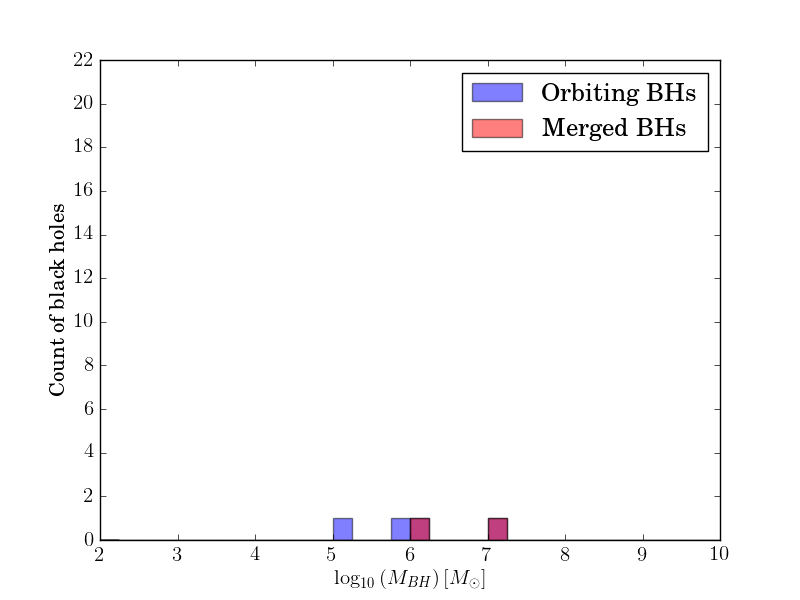
\includegraphics[width=0.45\textwidth]{plots/orbiting_bh_mass_histogram_gal_217.png}\\
\caption{default}
\label{default3}
\end{center}
\end{figure*}

\subsection{Mergers}
\begin{figure}[htbp]
\begin{center}
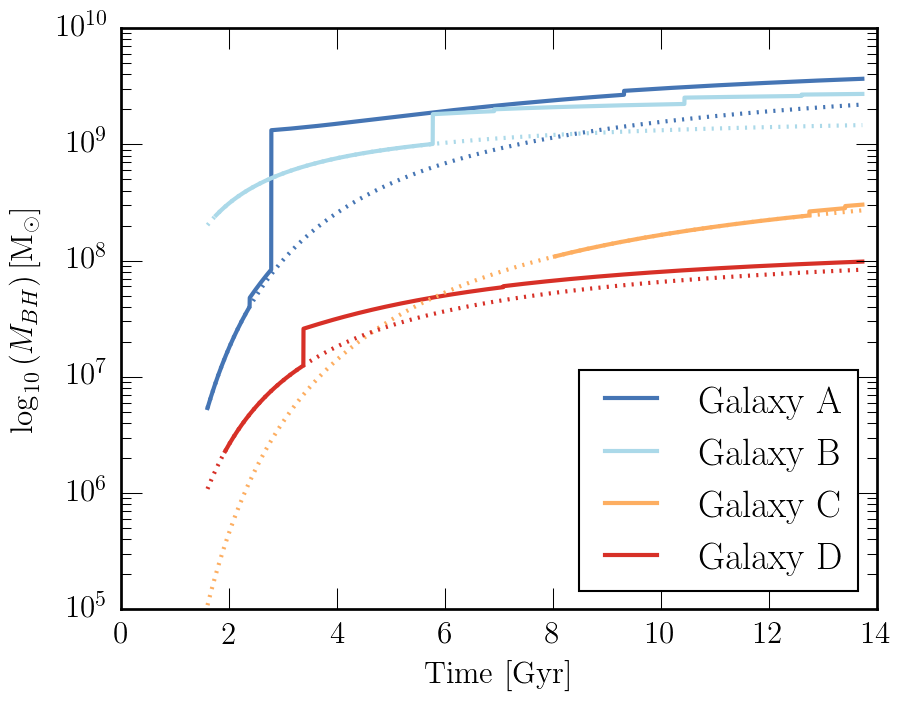
\includegraphics[width=0.45\textwidth]{plots/masses_ABCD.png}
\caption{default}
\label{default4}
\end{center}
\end{figure}



Note to work on:
\noindent A: two mergers early on, and then two more at around 10-12 Gyr
B: 4 mergers across the final 8 Gyr
C: two mergers in the final Gyrs
D: ?


\subsection{Ejections}
No complete ejections, but kicks to higher energy orbits.
\noindent A: one in a three-body encoutner\\
B: 7-ish kicks, some in nearly 4-body encounters\\
C: none\\
D: ?\\

\subsection{Stalling SMBH binaries}
A: two periods of BH binary in center for > Gyr, up to 6 Gyr\\
B: two short periods of BHBs\\
C: 2 classic BHB periods of about 1 Gyr each\\
D: ?

\subsection{Stalling SMBHs in the halo}
\begin{figure*}[htbp]
\begin{center}
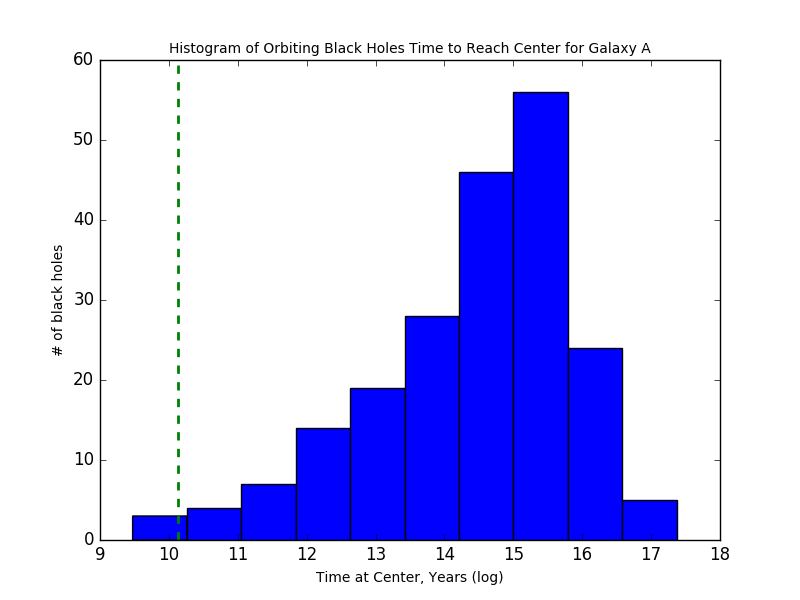
\includegraphics[width=0.45\textwidth]{plots/t_at_center_histogram_gal_1.png}
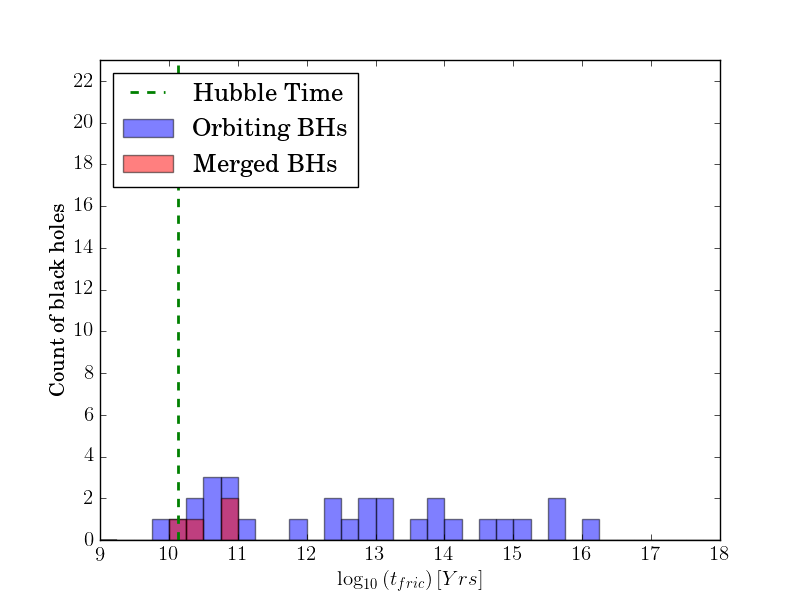
\includegraphics[width=0.45\textwidth]{plots/t_at_center_histogram_gal_65.png}\\
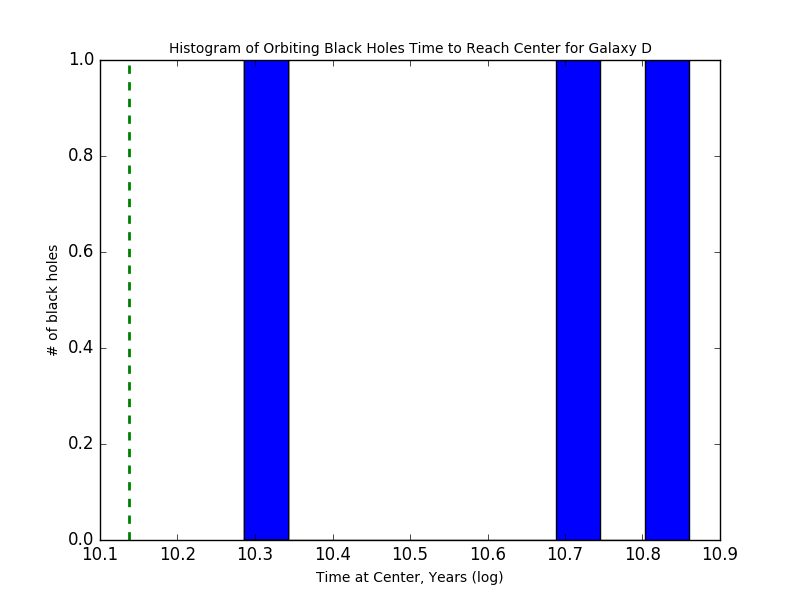
\includegraphics[width=0.45\textwidth]{plots/t_at_center_histogram_gal_187.png}
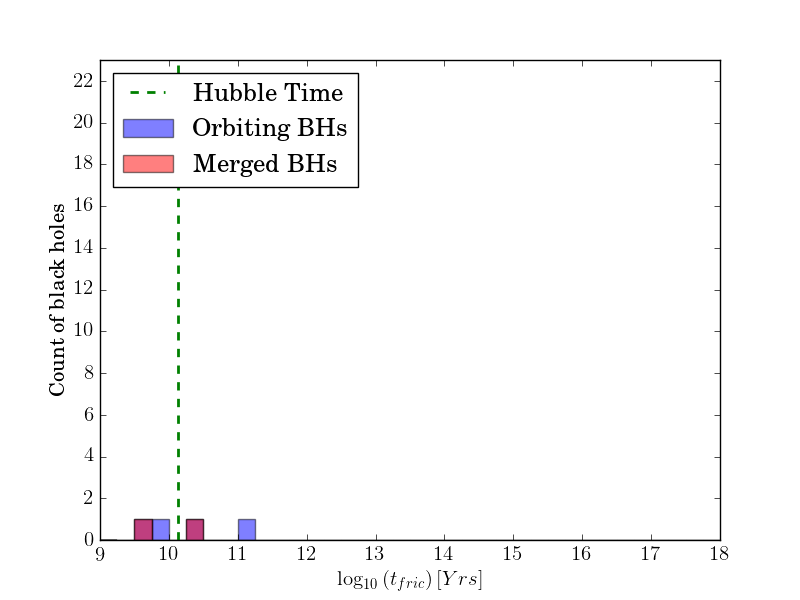
\includegraphics[width=0.45\textwidth]{plots/t_at_center_histogram_gal_217.png}\\
\caption{default}
\label{default5}
\end{center}
\end{figure*}

A: 95\% never make it into the central kpc\\
B: still about 90\% are in the halo\\
C: \\
D: ?



\section{Conclusions}\label{sec:conclusions}
What do we want to say?



\section*{Acknowledgements}

The authors would like to thank Andrea Kulier and Claire Lackner for providing merger tree data. AHWK acknowledges support by NASA through Hubble Fellowship grant HST-HF-51323.01-A awarded by the Space Telescope Science Institute, which is operated by the Association of Universities for Research in Astronomy, Inc., for NASA, under contract NAS 5-26555. 

\bibliographystyle{apj}
\bibliography{biblio}

%\begin{thebibliography}{}

%\bibitem[\protect\citeauthoryear{Aarseth}{2003}]{Aarseth03}
%Aarseth, S.~J., 2003, Gravitational N-Body Simulations (Cambridge University Press)


%\bibitem[\protect\citeauthoryear{K{\"u}pper et al.}{2011}]{Kupper11} 
%K{\"u}pper, A.~H.~W., Maschberger, T., Kroupa, P., Baumgardt, H., 2011, MNRAS, 417, 2300 

%\end{thebibliography}
\end{document}

